% !TEX root = /home/fred-olav/afgv/src/preamble.tex
\input preamble.tex
\huge
\centerline{\bf Heldagsprøve Gand reguleringsstasjon 23/24}  \bigskip
\normalsize
\vskip 1cm 
Kompetansemål:
\begin{itemize}[noitemsep]

	\item Prøven dekker alle kompetansemål i automatiseirngsfaget fra VG1 til VG3 auto.  
\end{itemize}

Alle ark som leveres inn skal ha elevens navn. \\ 

\newpage
\vskip 5pt 
\oppgave{}%7
% Elektroteknikk
\textbf{a)}\\
Programmer denne simuleringsfunksjonen for et temperaturreguleringssystem i et PLS program
\vskip 1cm 

$$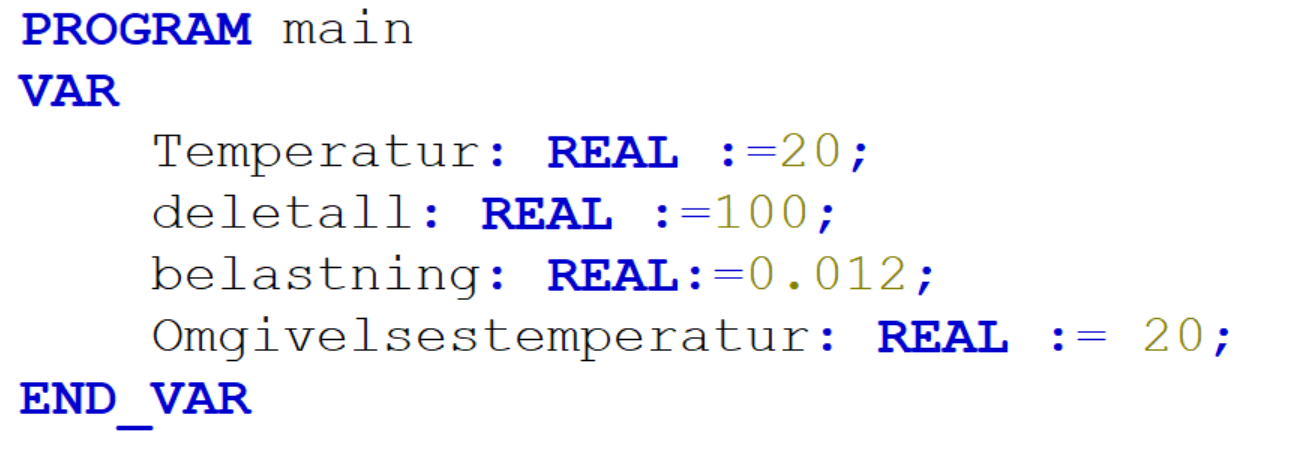
\includegraphics[width=15.5cm]{./aReg2324x05}$$
$$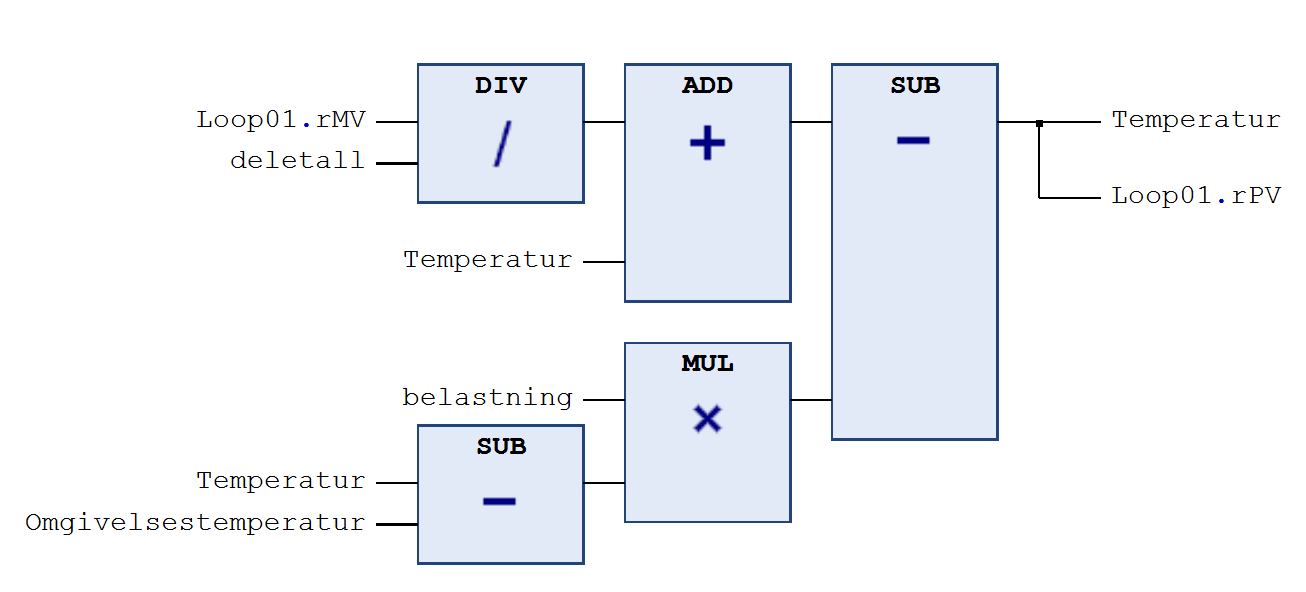
\includegraphics[width=15.5cm]{./aReg2324x06}$$

\textbf{b)}
Utvid programmet med en PID regulator som kan regulere simuleringsmodellen
\vskip 1cm 
\textbf{c)}
Programmer to skalleringsfunksjoner for temperaturtransmitter og reguleringsventil som tilkobles h.h.v. Wago 750-455 (AI 0-32760) og 750-555 (AO 0-32767). Disse to nettene skal kommenteres ut slik at de ikke er aktive i programmet. 
\vskip 1cm 

\oppgave{}%8
% Elektroteknikk
\textbf{a)}\\
\vskip 1cm 
Du skal lagen HMI styring til reguleringen av den simulerte modellen av et temperaturreguleringssystem. Det skal bestå av tre bilder:
\begin{itemize}
	\item Hovedmeny
	\item L3 P \& ID "bilde" av prosessen
	\item L4 Optimaliseringsbilde av prosessen
\end{itemize}

På L3 bildet skal det byttes faceplate når en hoder musen over ventilen. 


$$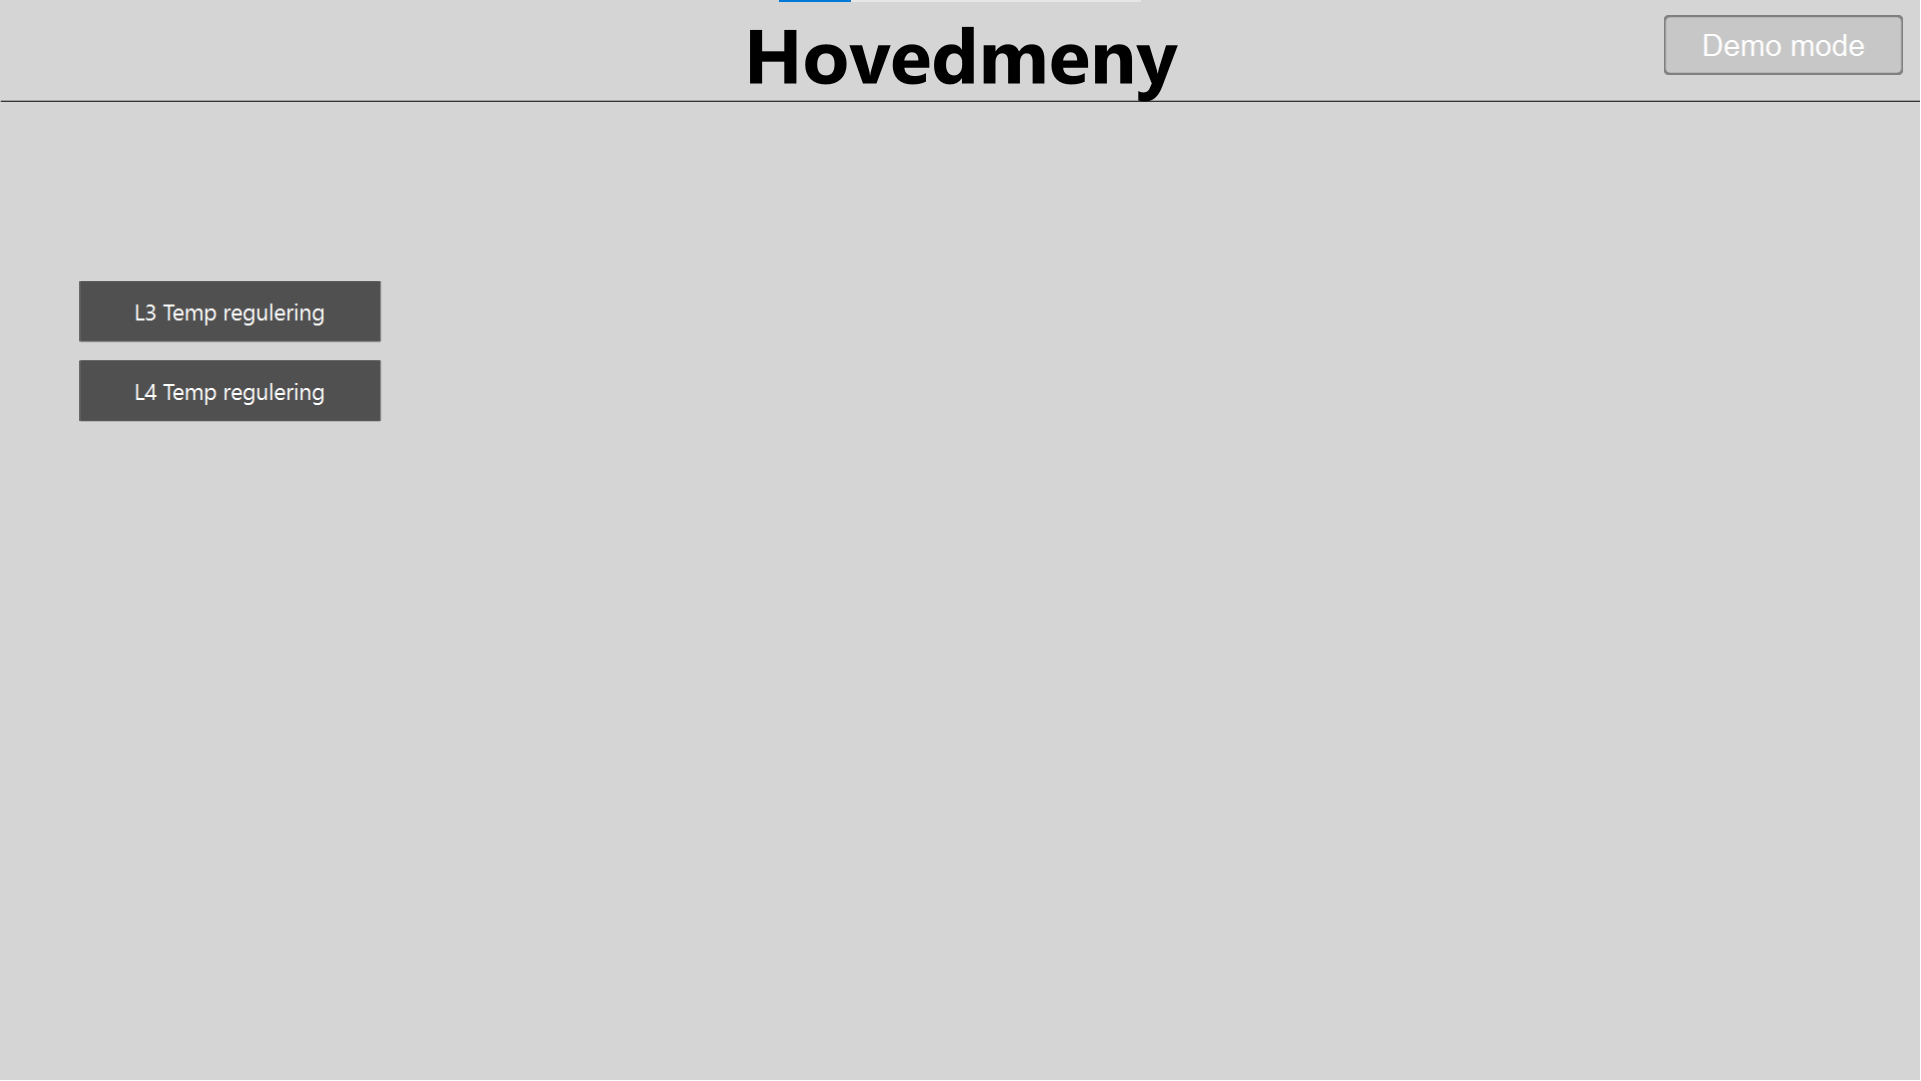
\includegraphics[width=15.5cm]{./aReg2324x03}$$
$$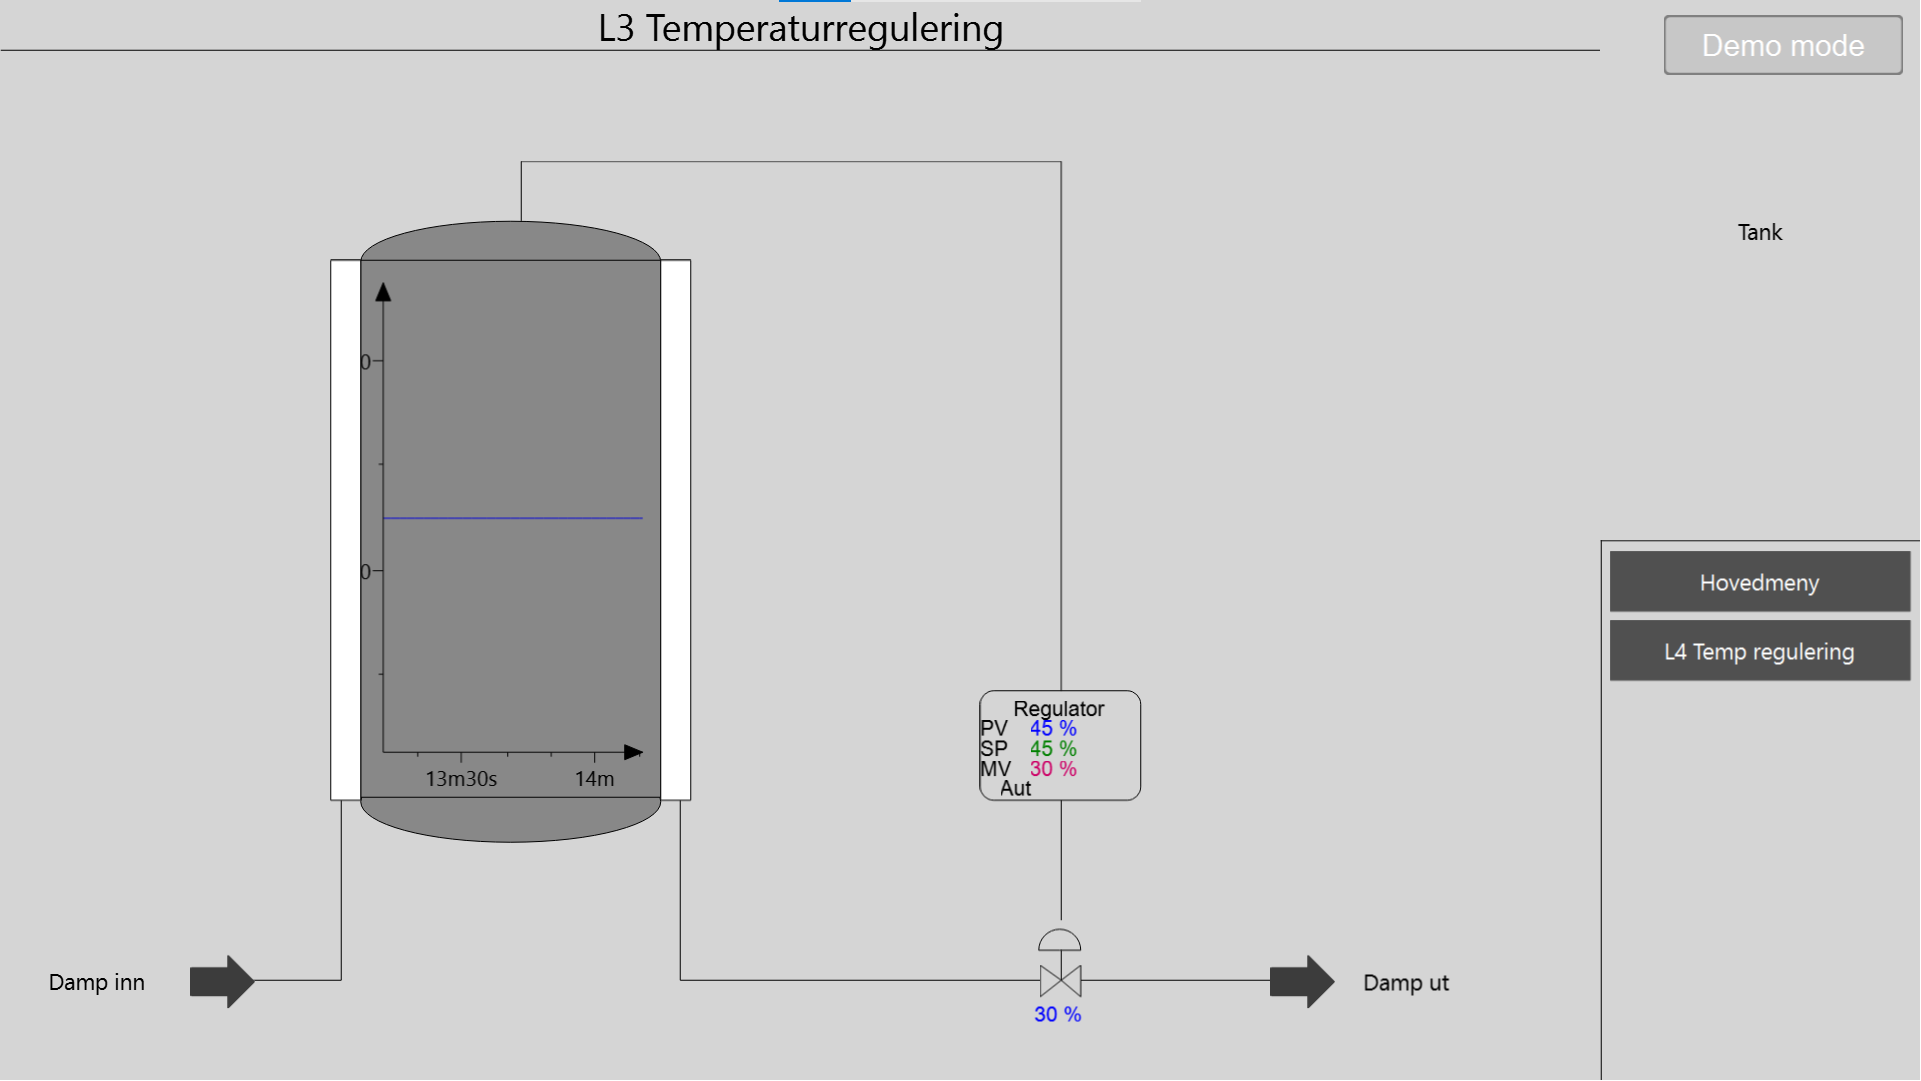
\includegraphics[width=15.5cm]{./aReg2324x02}$$
$$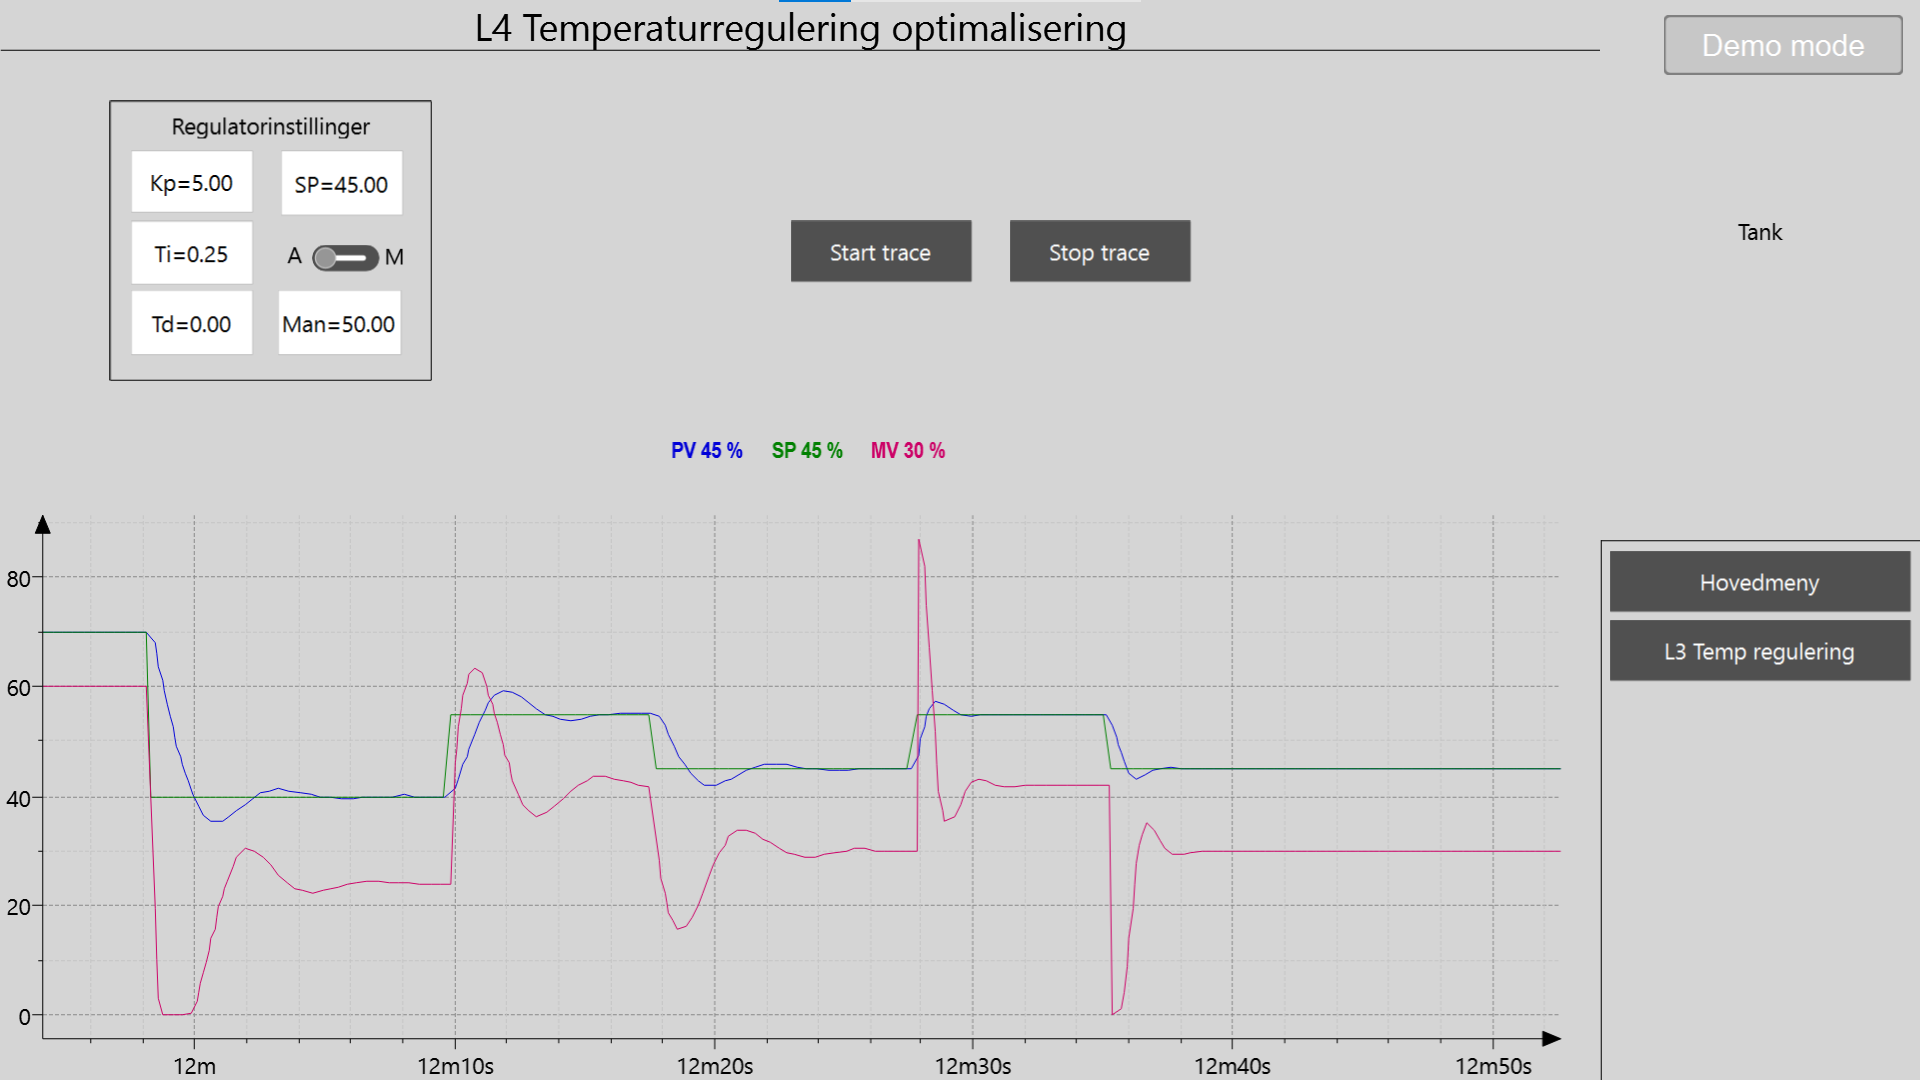
\includegraphics[width=15.5cm]{./aReg2324x01}$$

\vskip 2cm
\oppgave{}%9
Vis hvordan du kan optimalisere prosessen fra forrige oppgave. Bruk screenshot for å vise alle verdier du henter fra HMI. \\
Om du ikke har noe program fra forrige oppgave må du tegne og forklare hvordan du ville gått frem. 
\vskip 2cm
\oppgave{}%9
% Elektroteknikk
Du har fått i oppdrag i å montere og koble opp (ikke programmere) et Wago TP600 (delenummer 762-5306/8000-0002, size 10") touchpanel. i\\
Vis hvordan du ville planlagt, gjennomført og dokumentert oppdraget.
\vskip 2 cm 
Dokumentasjon på panelet sende til den epost når prøven starter. 

%\includepdf[pages=-,angle=90]{../eq/afgvformler.pdf}
\end {document}
